\chapter{Results}\label{CH:results}

We analyze the Torchbearer system on two fronts: first, we examine the differences between pipelines on a performance and efficiency level, comparing execution cost, execution time and similarity between results. Second, we perform a field study with real drivers using the Torchbearer system to navigate an unknown route, comparing cognitive load, driving performance and perceived task difficulty between all four pipelines and a control. Our aim with these analyses is to understand the effectiveness of human versus machine methodologies for landmark selection and to determine the efficacy of the overall system for improving drivers' cognitive load and performance during naivgation.

\section{Pipeline Comparison}

To evaluate the differences in efficiency, cost and solution overlap we created a test set of 400 maneuver points in San Francisco, California, using an existing dataset \cite{sfIntersections} of geographic coordinates for all intersections in the city. Maneuver points were created at random by selecting an intersection and a route leading into it; the bearing for maneuver point was computed by measuring the angle between the two points closest to the intersection in a poly line representation of the route (see \ref{fig:polyline}).

\begin{figure}[htbp]
  \centering
  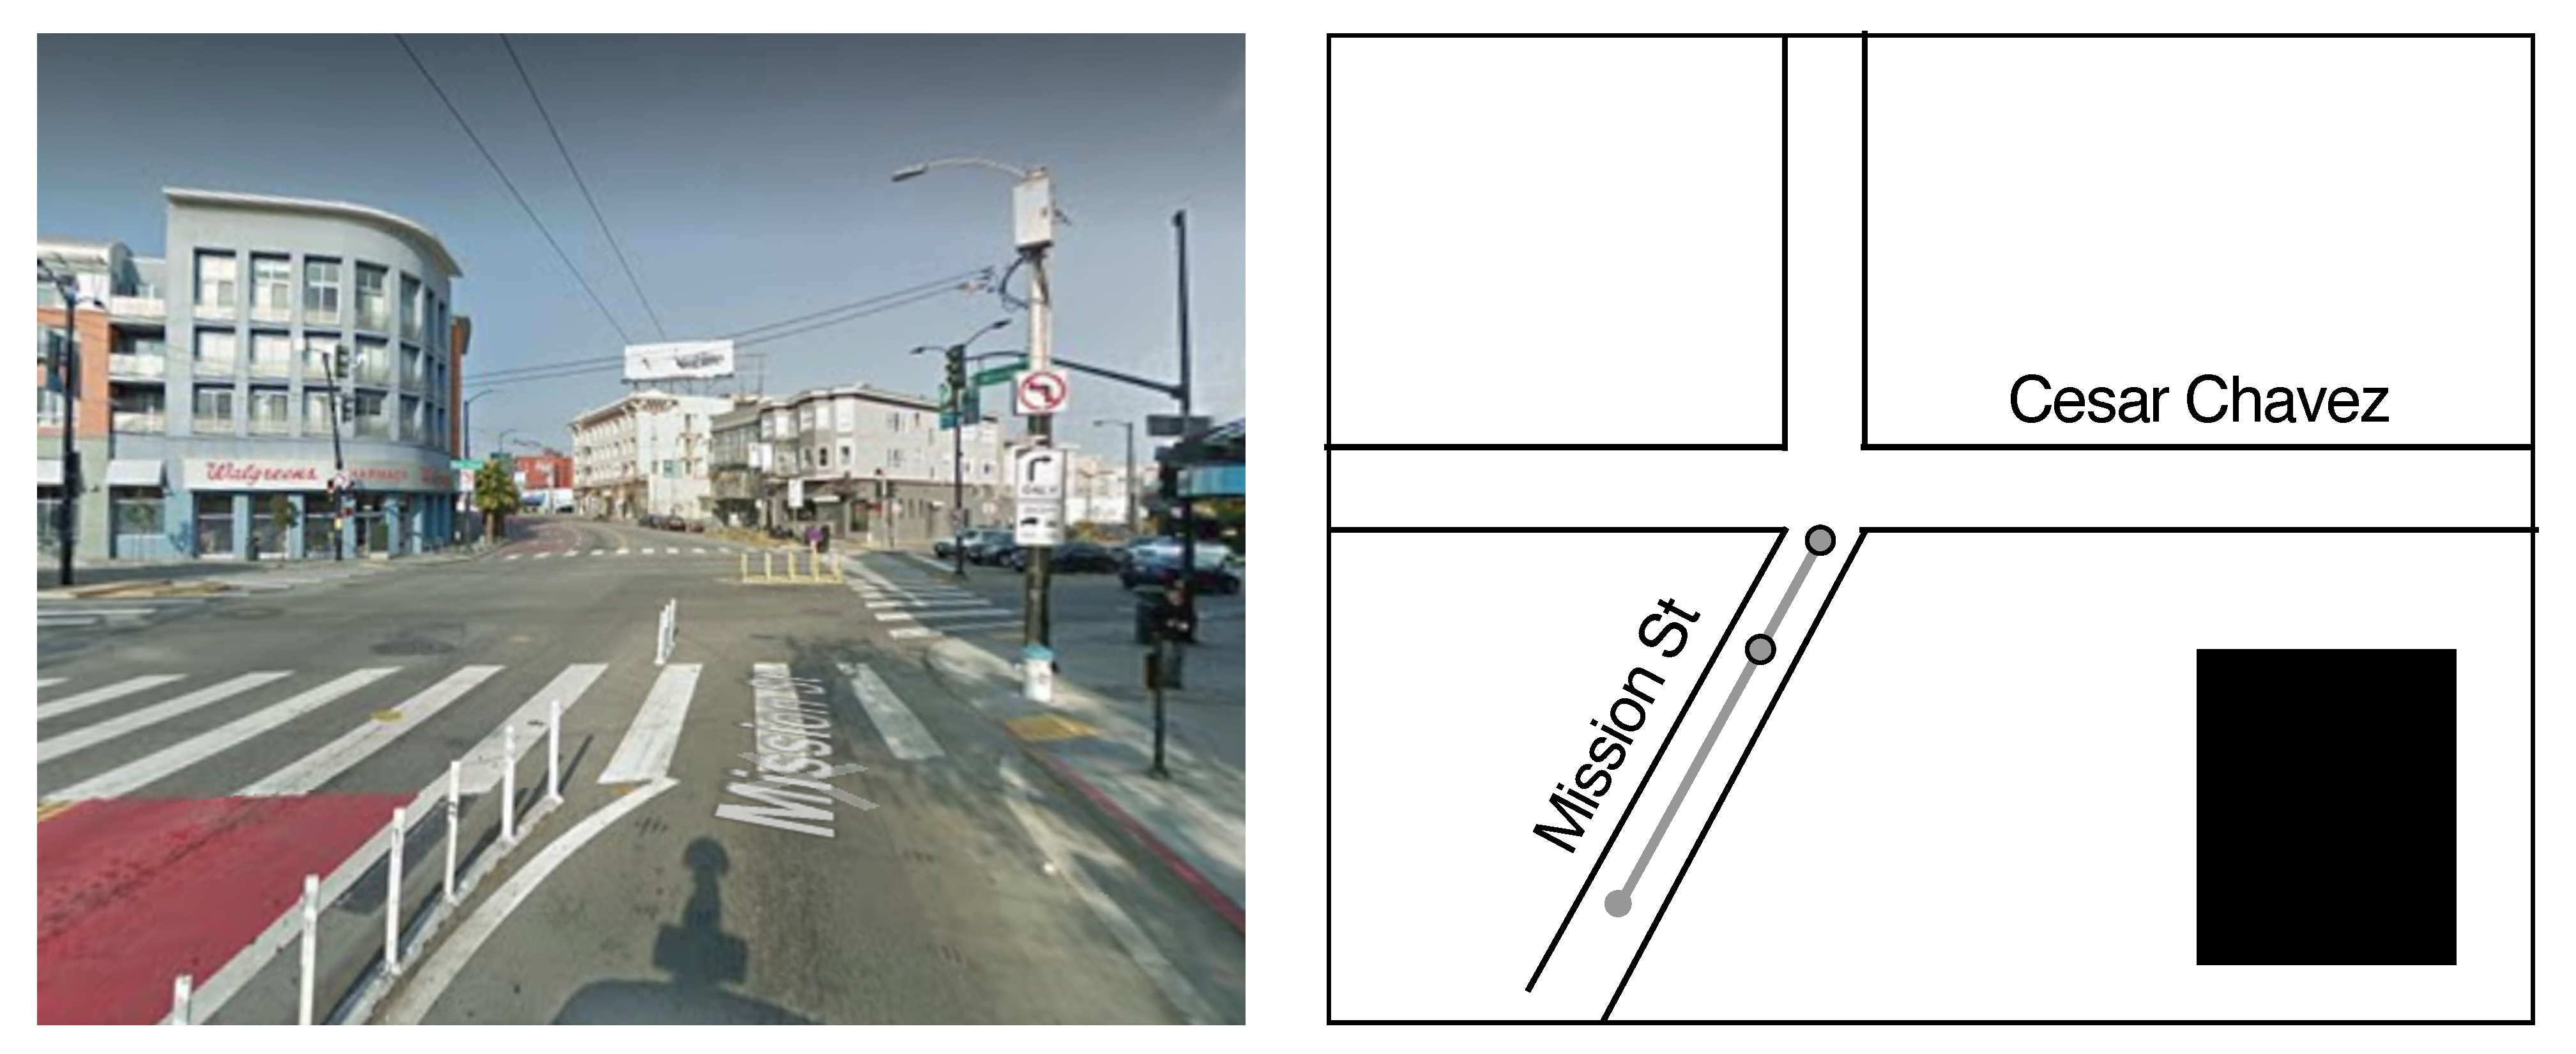
\includegraphics[width=0.6\textwidth]{images/POLYLINE.pdf}
  \caption{A hypothetical intersection in the SF test set. The grey line is a polyline representative of the selected route leading into the intersection. To find the bearing for the bearing value for the Torchbearer maneuver point we calculate the angle w.r.t. due north between the two points outlined in black.}
  \label{fig:polyline}
\end{figure}

Each maneuver point was processed through each of the four Torchbearer pipelines, resulting in a balanced result set of 1,600 pipeline executions.

\subsection{Marginal Cost}

Torchbearer pipelines incur monetary cost when they use MTurk to gather human input. In an effort to compare the drawbacks and benefits of each pipeline, it is important to have an understanding of the differences in expenditure.

The cost incurred for the processing of each maneuver point is recorded in the Torchbearer database as the pipeline executes; anytime a HIT is submitted to MTurk the cost is increased by $nc$ where $n$ is the number of workers who will complete the HIT and $c$ is the amount to be paid to each worker. For this experiment we paid workers \$0.0.5 for a saliency selection HIT, \$0.05 for a landmark description HIT and \$0.03 for a landmark verification HIT. These amounts were selected based on observational analysis of Mechanical Turk pricing for similar object-detection-related tasks; we aimed to offer above average pay for each type of HIT to avoid low pay as a confounding variable in work quality. The marginal pipeline costs (the cost of processing an additional maneuver point) are shown in \ref{fig:plot:cost}

\begin{figure}[htbp]
  \centering
  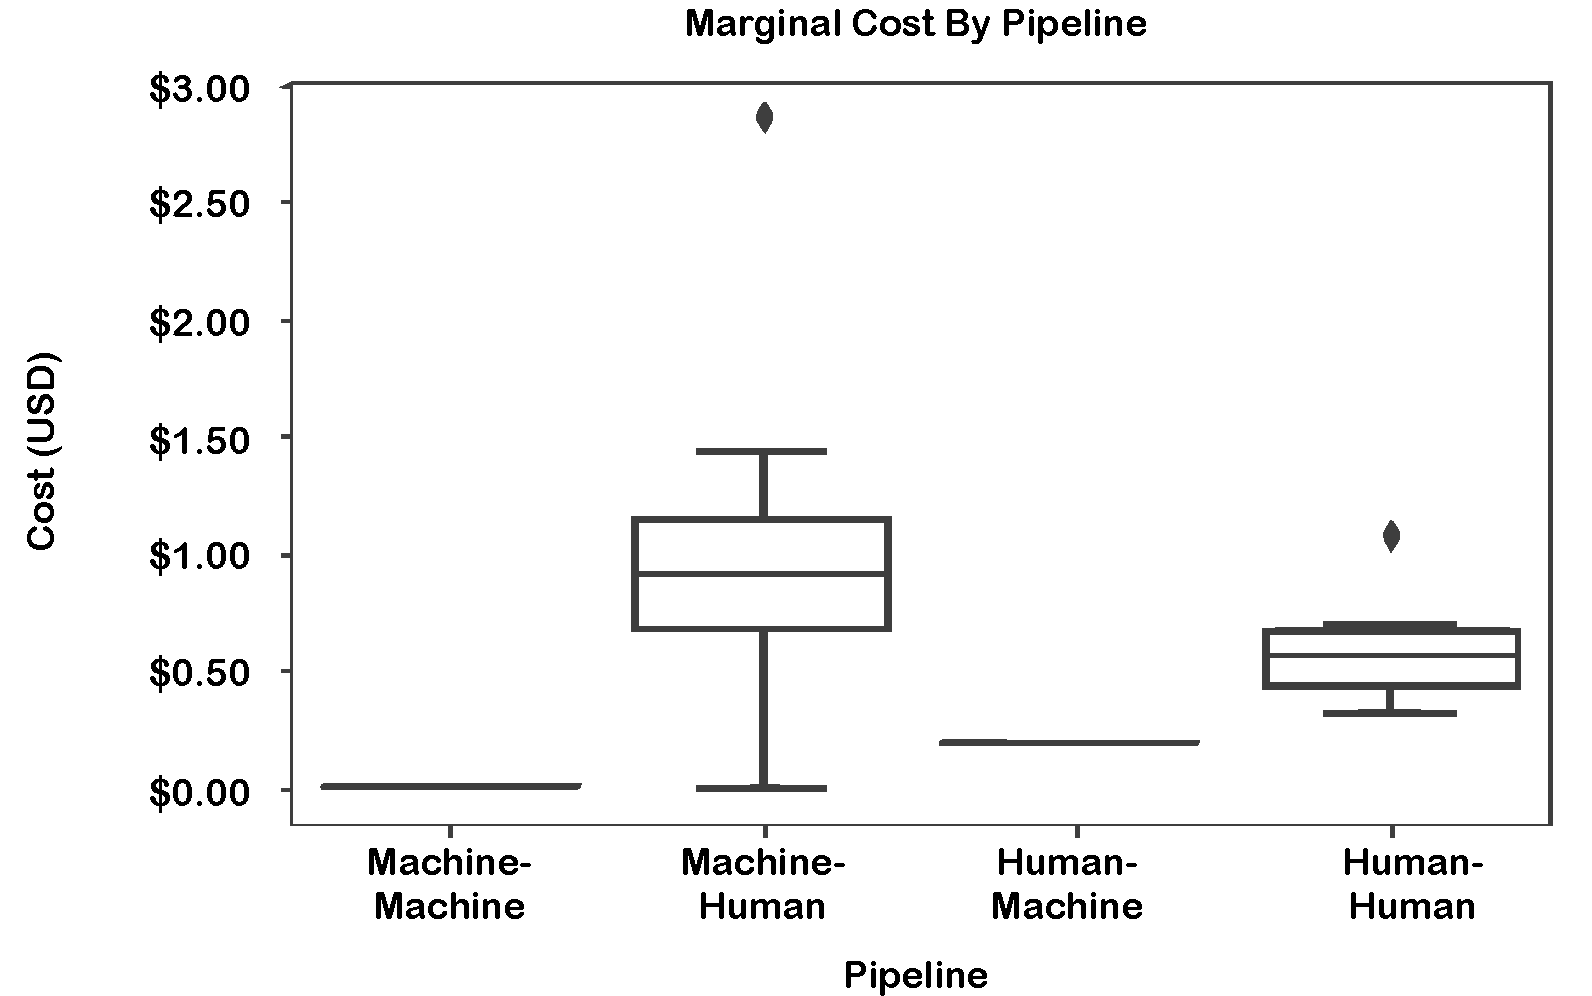
\includegraphics[width=0.6\textwidth]{images/plot_cost.pdf}
  \caption{}
  \label{fig:plot:cost}
\end{figure}

The marginal cost of the Machine-Machine pipeline is \$0.00, with no variance, since of course this pipeline makes no requests of human workers. The results for the Human-Machine pipeline are similarly deterministic---this pipeline requests a single saliency detection HIT with a fixed number of worker assignments (5 in our experiment). The Machine-Human pipeline exhibits not only the highest average cost, but also the highest variance. It is likely that both of these traits are due to the description verification component, which has the potential to repeat the entire description step, introducing non-determinism and increasing the cost of a execution significantly. 

This non-determinism due to verification is also a likely explanation of the variance observed in the Human-Machine pipeline. However, variance is less than the Machine-Human pipeline, which we attribute to humans' seeming ability to select more meaningful landmarks during the saliency step than the SalNet-based saliency approach. In other words, it is possible that the machine approach to saliency sometimes selects salient regions which do not contain an object that can be easily described, and contention is created among and between the describing workers and verification workers. This leads to more "loops" of the description step and a higher execution cost.

\subsection{Execution Time}
Along with monetary cost, execution time is a cost to using a given pipeline. Using our San Francisco test set, we measure both end-to-end processing time and task-wise execution time.

\subsubsection{End-to-End Execution Time}
We record the start and end timestamps for each execution; the difference between these timestamps are shown in \ref{fig:plot:executiontime}

\begin{figure}[htbp]
  \centering
  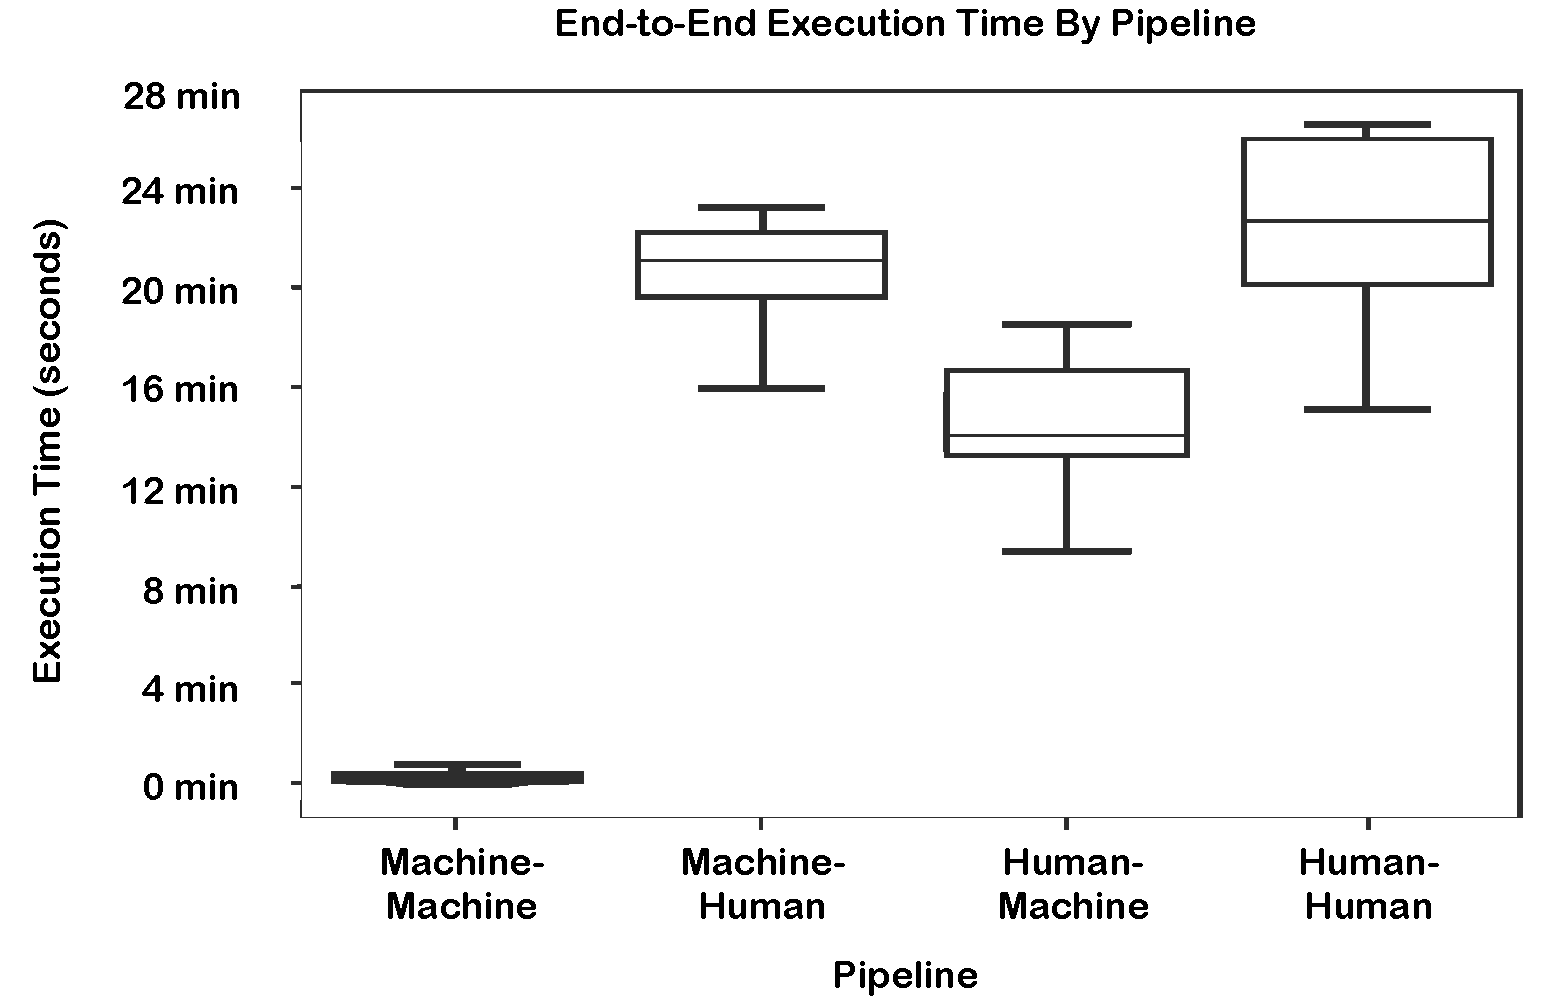
\includegraphics[width=0.6\textwidth]{images/plot_executiontime.pdf}
  \caption{}
  \label{fig:plot:executiontime}
\end{figure}

The Machine-Machine pipeline exhibits the lowest mean end-to-end execution time by an extreme margin, with very low variance. The pipelines which incorporate human input are, unsurprisingly, slower on order of tens of minutes. They also also exhibit significant variance, which is expected given the relative unpredictability of the human element. Likely for the same reasons we observe a higher marginal cost, we see a longer mean execution time for the Machine-Human pipeline than we do for the Human-Machine pipeline. The Human-Human pipeline has the largest variance, due to the most reliance on human work, and also the highest time. It is interesting to note that the mean time of the Human-Human pipeline is not much higher than that of Machine-Human, implying that the human saliency detection task is relatively fast compared to the human description task.

\section{Field Experiments}

To evaluate the efficacy of each of our approaches for reducing driver cognitive load and improving driving performance, we conduct a naturalistic driving study (real driver, real vehicles, real roads) in which subjects navigate an unknown route using the Torchbearer system. It must be noted up front that, due to constraints on time and resources, a full-scale human factors study is out of the scope of this work. While the experimental design we discuss could be applied to a larger sample and yield significant results, here we use a sample size of only five human subjects. Along with contributing a experimental design for future work, this small-scale study provides anecdotal evidence as to the effectiveness of the Torchbearer system.

\subsectino{Experimental Design}

We evaluate each of Torchbearer's four pipelines against a control pipeline which delivers instructions containing no landmarks. The control pipeline is comparable to a mainstream navigation application, such as Google Maps, which provides only street names and distances in its instructions.

Five subjects drove an identical route through downtown Bozeman, Montana, using only the Torchbearer app for navigation. This route was divided into five legs, and a different pipeline was used for each leg. The subject was given no information about the route prior to the start of driving.